\documentclass{article}

% ML for Systems @ NeurIPS 2026: non-anonymous, 4-page strict limit
% (references and appendix do not count). Camera-ready: add ,final
\usepackage[dblblindworkshop]{neurips_2026}
\workshoptitle{Machine Learning for Systems}

\usepackage[utf8]{inputenc}
\usepackage[T1]{fontenc}
\usepackage{hyperref}
\usepackage{url}
\usepackage{booktabs}
\usepackage{amsfonts}
\usepackage{amsmath}
\usepackage{nicefrac}
\usepackage{xcolor}
\usepackage{graphicx}
\usepackage{placeins}
\graphicspath{{figures/}}

\title{GORGO: Online Tuning for Cross-Region Network-Aware LLM Serving}

\author{
  Alessio Ricci Toniolo \\
  Modal Labs \\
  \texttt{atoniolo@andrew.cmu.edu} \\
  \And
  Rome Thorstenson \\
  ART \\
  \texttt{rome@arcadiaresearch.team} \\
  \And
  Abinaya Dinesh \\
  ART \\
  \texttt{abinaya@arcadiaresearch.team} \\
}

\begin{document}

\maketitle

\begin{abstract}
Increasingly, LLM inference services proxy client requests to engine replicas distributed globally.
Load-balancing policies must jointly account for
factors including KV-cache locality, replica load, and variable network latency when
optimizing for metrics like latency and TTFT.
However, existing systems only evaluate a subset of these factors in their cost
model, leading to uneven concentrations of load and KV-cache across replicas. We
present GORGO, a proxy architecture that holistically factors network latency,
prefill cost, and queueing delay using tunable parameters. Since open-source chat
datasets such as LMSYS-Chat-1M and WildChat-4.8M lack long-context, high
prefix-reuse data, we publicly release a synthetic dataset, ART-Chat-2.5M, from
long-context production metadata. Intra-user prefix reuse and average token
length in ART-Chat-2.5M are 19$\times$ and 6$\times$ higher than in WildChat-4.8M. On a tuning window from ART-Chat-2.5M,
evolutionary strategies guide the GORGO policy's parameters to directly optimize
p95 TTFT. During a held-out evaluation window, we fix the parameter values learned
from tuning and improve p95 TTFT by 15.5\% and p95 end-to-end (E2E) latency by
30.9\% over baseline load-balancing policies such as simple session affinity
and prefix-cache.
\end{abstract}

% -----------------------------------------------------------------------
\section{Introduction}
\label{sec:intro}
% -----------------------------------------------------------------------

In LLM serving systems, perceived latency to the user is dominated by the time-to-first-token (TTFT). On a single replica, TTFT is dominated by three costs: (i) prefill time, (ii) round trip time (RTT) from client (proxy) to replica, and (iii) queueing delay behind in-flight requests. Prefix-caching, which is enabled in inference engines SGLang \citep{sglang2024} and vLLM \citep{vllm2023}, eliminates the prefill cost of previous turns in a multi-turn conversation. As LLM context windows increase in length, the time saved by prefix caching 90\% of a prompt with 100,000 tokens reduces the prefill cost to 10,000 tokens and decreases TTFT substantially.

Since LLM deployments proxy requests to inference engines across regions, the cost savings of prefix-caching depend on choosing a replica with the request session's prefix. Popular routing policies such as consistent hashing and prefix reuse aim to distribute load evenly while creating affinity between a session's requests and replica(s) to maximize KV-cache reuse \citep{karger1997consistent, chord2003, sglang2024, skywalker}. In compute-constrained regimes, bursty workloads can saturate a high-affinity replica, causing head-of-line (HOL) queueing delays from decode memory contention and negating cost savings from prefix-cache reuse. Routing policies that holistically evaluate all costs related to TTFT can maintain high prefix-cache reuse while minimizing the negative effects of load saturation and heterogeneous network latency.

Existing load balancing policies such as least-load, session affinity, and prefix-reuse may account for replica load or KV-cache hit rate; however, no existing policies consider network latency in cross-region scenarios, which can range on the order of 10ms to 1s (Appendix~\ref{app:setup}). GORGO's routing policy accounts for all three TTFT costs, normalizes the units of measurement via tunable parameters, and jointly optimizes parameters through online tuning on real user workloads. To tune and stress-test different routing policies, in (\S\ref{sec:characterization}) we compile an LLM traffic trace from real production requests with high prefix-reuse and long-context prompts. The trace follows Mooncake's FAST'25 format \citep{qin2024mooncake} containing per-request timestamps, which can be linearly scaled to simulate different load profiles for various hardware. On a held-out window, fixed-weight GORGO improves p95 TTFT by 15.5\% and p95 E2E latency by 30.9\% over session affinity (\S\ref{sec:results}).

% -----------------------------------------------------------------------
\section{GORGO}
\label{sec:method}
% -----------------------------------------------------------------------

\subsection{Design space}

For LLM load balancing policies, the design space includes which routing signals to consider and methods for choosing environment settings.

\textbf{Routing signals}: Across existing load balancing policies, two distinct routing signals are considered: (i) replica load and (ii) KV-cache locality.
Simple policies such as least-load and least-request aim to evenly balance replica load while prefix-cache and simple-session-affinity aim to maximize KV-cache reuse per request.
NVIDIA Dynamo~\citep{nvidiaDynamoRouter}, SGLang Router~\citep{sglang2024}, and Preble~\citep{preble} offer algorithms that jointly optimize for replica load and KV-cache locality.

GORGO takes inspiration from early content-delivery network design, which has many similarities to LLM serving.
\citet{wang2002cdn} used three signals---server load, network proximity, and cache locality---to reduce response time and increase capacity. Evaluating network proximity can improve
responsiveness, or TTFT, in geo-distributed serving environments. GORGO is the first LLM load balancing policy to also optimize (iii) network latency from client to server.

\textbf{Weight-selection methods}: Methods for tuning the weights of a request scheduler fall into (i) offline and (ii) online protocols.
Existing offline methods include Dynamo's SLA Planner, which has a sophisticated method to autoscale prefill and decode workers to meet TTFT and ITL targets.
It requires profiling before deployment to determine the optimal tensor parallelism configurations and scaling parameters for the planner to use during runtime~\citep{nvidiaDynamoPlanner}.

GORGO uses online calibration because cache state, queue state, and batching behavior are intrinsically influenced by the routing policy's decisions, and accurately replicating the conditions necessary to evaluate the policies requires a dedicated replay fleet, shadow execution, or a sufficiently accurate simulator of cache and continuous-batching dynamics.
After all, a request log generated under one policy does not contain the counterfactual cache and queue evolution that would have arisen under another set of weights.

\subsection{Cost model}

TTFT is known to consist of three different costs: network latency, prefill time, and queueing delay \citep{banaserve2025}. The KV-Cache, which stores key-value pairs of input sequences, removes redundant prefill computation for user sequences sharing a prefix with previously computed sequences \citep{sglang2024}. In a cross-region deployment setting, for an inference engine replica $i$ holding a set of cached token prefixes $c_i$, the cost of TTFT can be defined as the following function, where $x_r$ is the input sequence of tokens for a request $r$ and the prefill time depends only on the set difference $(x_r \setminus c_i)$, the tokens in $x_r$ not already cached on $i$:

\begin{equation}
\mathrm{TTFT} = T_{\texttt{network}}(i) + T_{\texttt{queue}}(i) + T_{\texttt{prefill}}(x_r \setminus c_i)
\label{eq:ttft}
\end{equation}

Theoretically, $T_{\texttt{network}}$ and $T_{\texttt{queue}}$ correspond with round trip time from a client to server and the duration of request processing ahead of the incoming request $r$. However, inference engines support batching requests continuously~\citep{orca2022}, and admission is still bounded by a maximum number of concurrent requests and the available KV-cache budget~\citep{vllm2023}.

In a distributed system, the temporal delay of retrieving queueing metrics from an engine replica makes cost evaluation challenging. We represent the input to $T_{\texttt{queue}}$ as the total number of tokens of requests without a completion event on the client proxy. $T_{\texttt{network}}$ is measured trivially as the exponential weighted moving average of a ping's round trip time from client proxy to server.
\begin{equation}
\mathrm{TTFT} = T_{\texttt{network}}(\mathrm{RTT}_i) + T_{\texttt{queue}}\left(i, \sum_{j=1}^{n_r} x_j\right) + T_{\texttt{prefill}}(x_r \setminus c_i)
\label{eq:ttft-proxy}
\end{equation}

\subsection{GORGO proxy design}

The GORGO proxy routes client requests to the engine replica with the minimum calculated cost from Equation~\ref{eq:ttft-proxy}, parameterized by weights $W_{\texttt{rtt}}$, $W_{\texttt{prefill}}$, and $W_{\texttt{queue}}$. These parameters weight the inputs $T_{\texttt{network}}$, $T_{\texttt{queue}}$, and $T_{\texttt{prefill}}$, which unfairly mixes the units of time and tokens, to normalize the correlated costs of latency, prefill cost, and queueing time on TTFT. The weight of $T_{\texttt{prefill}}$ is fixed to 1 because GORGO proxy makes routing decisions based on relative replica cost: only the ratio of weights matters in this design.
\begin{equation}
\mathrm{TTFT} = W_{\texttt{rtt}} * T_{\texttt{network}}(\mathrm{RTT}_i) + W_{\texttt{queue}} * T_{\texttt{queue}}\left(i, \sum_{j=1}^{n_r} x_j\right) + T_{\texttt{prefill}}(x_r \setminus c_i)
\label{eq:score}
\end{equation}

GORGO proxy uses a simple (1+1) evolutionary strategy to tune weights $W_{\texttt{rtt}}$ and $W_{\texttt{queue}}$ on the objective function, p95 TTFT.
Each parent weight $x_{t,k}$ is perturbed multiplicatively in log-space by a normal random variable $z_k$ times step size $\sigma$, and the new offspring weight $x_k'$ is clamped to values in the hyperparameter range $[lo_k, hi_k]$ where $lo_k > 0$ and $hi_k > 0$.

\begin{equation}
x_k' = \mathrm{clip}\left(\exp(\ln(x_{t,k}) + \sigma_t * z_k), [lo_k, hi_k]\right)
\end{equation}

When $x'$ beats the parent weight $x_t$ on the objective metric, the incumbent weight $x_{t+1}$ is updated to $x'$, and $\sigma$ is adjusted to maintain Rechenberg's 1/5 success rule~\citep{rechenberg1973} of roughly one accepted offspring for every five proposals.

% -----------------------------------------------------------------------
\section{Dataset}
\label{sec:characterization}
% -----------------------------------------------------------------------

Existing LLM chatbot datasets lack two critical components for benchmarking
cache-aware policies: (i) prefill-bound requests with long-context prompts and
(ii) multi-turn workloads with high prefix-reuse between requests. For example,
we measure the average request length and global prefix reuse of
\textbf{LMSYS-Chat-1M}~\citep{lmsys2024} and \textbf{WildChat-4.8M}~\citep{wildchat2024},
two popular LLM datasets derived from public chatbot demos
(Table~\ref{tab:datasets}).

\textbf{ART-Chat-2.5M} is a long-context, multi-turn dataset synthetically generated from
a week-long metadata trace of production inference traffic with the same
prefix-reuse structure as the original workload. We release a replay-ready trace
in the Mooncake FAST'25 format, which contains per-request timestamps, request
metadata, and synthetically generated chat completion data~\citep{qin2024mooncake}.
The dataset is included in the anonymous supplementary material.
By storing request timestamps, one can linearly scale the time between requests
to simulate different load profiles for various hardware. Notably, the intra-user prefix reuse and average token length in ART-Chat-2.5M
are 19$\times$ and 6$\times$ higher than in WildChat-4.8M. Dataset analysis is in Appendix~\ref{app:dataset}.

\begin{table}[t]
\centering
\small
\caption{Dataset. ART-Chat-2.5M contains higher average input tokens and global prefix reuse, which is measured by
adding the intra-user reuse and cross-user reuse, over other chat datasets.}
\label{tab:datasets}
\begin{tabular}{lrrrrr}
\toprule
Dataset & Total reqs & Users & Avg input tokens & Intra-user reuse & Global reuse \\
\midrule
LMSYS-Chat-1M & 1{,}000{,}000 & --- & 467 & --- & 3.4\% \\
WildChat-4.8M & 3{,}199{,}860 & 1{,}833{,}730 & 2{,}925 & 4.7\% & 32.5\% \\
ART-Chat-2.5M & 2{,}525{,}215 & 4{,}984 & 17{,}964 & 89.4\% & 89.7\% \\
\bottomrule
\end{tabular}
\end{table}

% -----------------------------------------------------------------------
\section{Results}
\label{sec:results}
% -----------------------------------------------------------------------

\paragraph{Results across two windows.}
We evaluate on a three-region fleet of L40S GPUs running Qwen3.5-35B-A3B in the SGLang inference engine (baselines and windows in Appendix~\ref{app:setup}). GORGO tunes $w_{\mathrm{rtt}}$ and $w_{\mathrm{queue}}$ on Apr~5 to minimize rolling p95 TTFT, then freezes the learned weights ($w_{\mathrm{rtt}}{=}0.276$, $w_{\mathrm{queue}}{=}0.5$) on Apr~6 (Apr~7 in Appendix~\ref{app:apr7}).

\begin{table}[ht]
\centering
\small
\caption{Experiment results. In the tuning window, GORGO learns weights $w_{\mathrm{rtt}}{=}0.276$, $w_{\mathrm{queue}}{=}0.5$ after initializing
at weights $w_{\mathrm{rtt}}{=}0.5$, $w_{\mathrm{queue}}{=}0.1$. On the held-out evaluation window, GORGO's weights are frozen, and
the policy outperforms every baseline policy on p95 TTFT.}
\label{tab:results}
\setlength{\tabcolsep}{2.7pt}
\begin{tabular}{lrrrrrrr}
\toprule
Policy & TTFT p50 (ms) & TTFT p95 & TTFT p99 & E2E p50 (s) & E2E p95 & E2E p99 & ITL (ms) \\
\midrule
\multicolumn{8}{l}{\textit{Tuning window --- Apr~5 16:15--16:45 (7{,}195 requests)}} \\
\midrule
\textbf{GORGO}          & \textbf{673} & 2{,}514          & 4{,}473          & \textbf{3.04}  & \textbf{8.91}  & \textbf{17.54} & \textbf{17.6} \\
simple-session-affinity & 712          & \textbf{2{,}428} & 5{,}190          & 3.48           & 18.27          & 22.61          & 20.2 \\
least-load              & 763          & 2{,}447          & \textbf{4{,}349} & 3.63           & 13.69          & 17.57          & 21.7 \\
least-request           & 968          & 3{,}970          & 7{,}012          & 4.37           & 16.62          & 20.81          & 25.2 \\
prefix-cache            & 1{,}477      & 6{,}784          & 9{,}613          & 13.14          & 22.63          & 26.81          & 82.3 \\
\midrule
\multicolumn{8}{l}{\textit{Held-out eval --- Apr~6 15:05--15:35 (7{,}630 requests)}} \\
\midrule
\textbf{GORGO}          & \textbf{491} & \textbf{1{,}584} & \textbf{2{,}222} & \textbf{1.80}  & \textbf{3.28}  & \textbf{4.37}  & \textbf{9.0} \\
simple-session-affinity & 627          & 1{,}875          & 3{,}056          & 2.01           & 4.75           & 7.34           & 10.3 \\
least-load              & 616          & 1{,}818          & 2{,}885          & 2.17           & 4.06           & 5.78           & 10.7 \\
least-request           & 634          & 1{,}852          & 2{,}484          & 2.08           & 3.99           & 5.23           & 9.9 \\
prefix-cache            & 574          & 1{,}798          & 2{,}750          & 2.07           & 4.95           & 10.34          & 10.6 \\
\bottomrule
\end{tabular}
\end{table}

While the GORGO policy's weights are
updated to minimize p95 TTFT during tuning, the held-out, fixed-weight evaluation
shows generalization of the learned values across days, with GORGO improving p95
TTFT by 15.5\% and E2E latency by 30.9\% over session-affinity. GORGO
slightly underperforms baseline policies on the tuning window because the
evolutionary strategy actively explores the space of parameters and tests worse weights than the learned solution, which converges after 672 samples
(Appendix~\ref{app:es}).

\paragraph{BFCL multi-turn replay.}
As an additional high-prefix-reuse workload, we replay 200 teacher-forced
episodes from BFCL's \texttt{multi\_turn\_base} subset, where each episode
contains sequential tool calls~\citep{patil2025bfcl}. We use two Qwen3-4B H200
replicas in us-east and us-west, 128 concurrent episodes, and at most 256 output
tokens per request.

\begin{table}[ht]
\centering
\small
\caption{BFCL multi-turn replay. Bold marks the best value per column.}
\label{tab:bfcl}
\setlength{\tabcolsep}{2.7pt}
\begin{tabular}{lrrrrrrr}
\toprule
Policy & TTFT p50 (ms) & TTFT p95 & TTFT p99 & E2E p50 (s) & E2E p95 & E2E p99 & ITL (ms) \\
\midrule
\textbf{GORGO}          & \textbf{3{,}328} & \textbf{4{,}700} & 5{,}720          & \textbf{3.66} & \textbf{5.17} & \textbf{6.15} & --- \\
simple-session-affinity & 3{,}655          & 5{,}087          & \textbf{5{,}608} & 4.11          & 5.61          & 6.17          & --- \\
\bottomrule
\end{tabular}
\end{table}

Under high load, GORGO reduces p50 and p95 TTFT by 8.9\% and 7.6\%, and p50
and p95 E2E latency by 10.8\% and 7.9\%, respectively.

\paragraph{Exploiting continuous batching in SGLang.}
In the continuous batching paradigm, GORGO can stumble upon abnormal weight values and achieve an impressively low p95 TTFT at the cost of high p95 E2E latency.
Appendix~\ref{app:load_ablation} presents results from an experiment where the evolutionary strategy learns to set $w_{\mathrm{queue}}$
to 0 while keeping $w_{\mathrm{rtt}}$ near 0.23, which results in p95 TTFT 17\% better than the next-best policy. For this window,
GORGO chose to send 100\% of requests to the closest replica in us-ashburn. Once the request enters the memory-bound decode phase, the replica's memory headroom saturates, KV-cache thrashes between GPU and CPU memory, and ITL/E2E latency collapses~\citep{orca2022, vllm2023}.
To mitigate this, we set a non-zero lower bound for the load-term, which forces the policy to balance request concentration across replicas.

\FloatBarrier
\bibliographystyle{plainnat}
\bibliography{references}

\clearpage
\appendix

\section{Experimental setup}
\label{app:setup}

\paragraph{Proxy and engine configuration.}
Each policy runs the GORGO proxy on a small CPU worker in us-ashburn and controls
a dedicated SGLang inference engine in each of the following regions: us-ashburn,
eu-frankfurt, and ap-seoul. The engines contain two L40S GPUs each and serve the
Qwen3.5-35B-A3B model in FP8 format~\citep{qwen3technical}. All policies are
benchmarked on the same workload in parallel to rule out any variance in network
conditions. The round-trip time between the us-ashburn proxy and engines during
the tuning window is plotted in Figure~\ref{fig:rtt}. Due to the Qwen model's
limited context length of 32{,}768 tokens, we filter out any requests that
contain $>$24{,}000 tokens to leave adequate KV headroom. In SGLang, we set
\texttt{max\_concurrent\_requests} to 64 and \texttt{max\_output\_tokens} to 128
to limit unnecessary decode while simulating adequate load on the replica. All
workloads run alongside the proxy, dispatching requests to a local chat
completion endpoint.

\begin{figure}[ht]
\centering
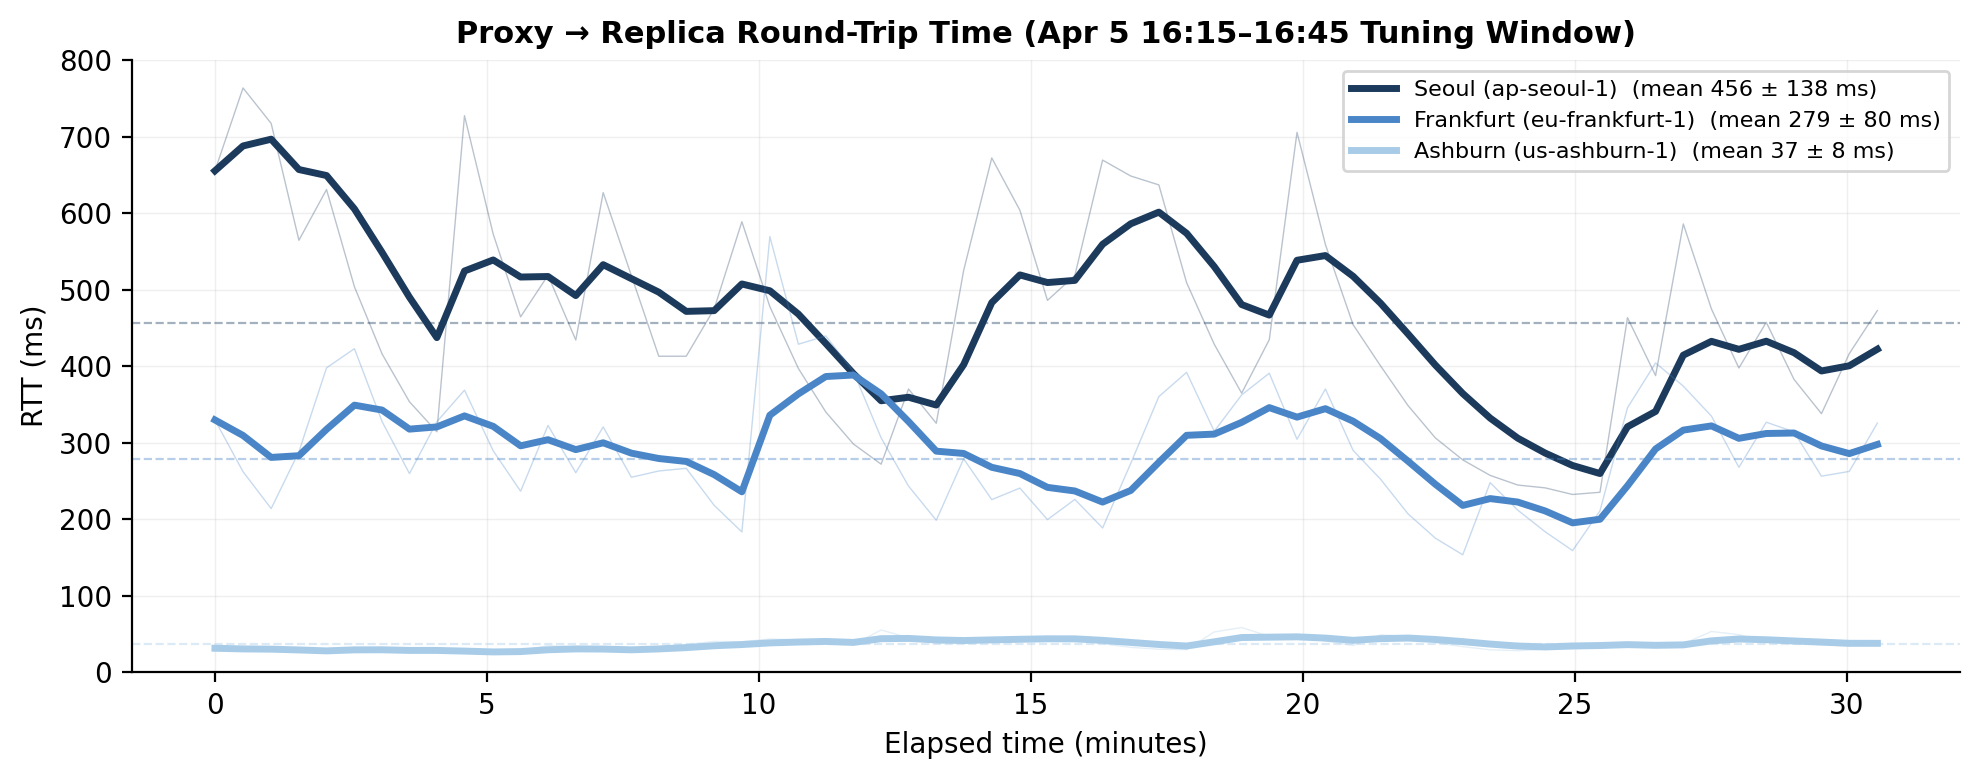
\includegraphics[width=\linewidth]{rtt_timeseries_apr5_1615_1645.png}
\caption{Round trip time (RTT) between the GORGO policy's proxy in us-ashburn and the SGLang engines in us-ashburn, eu-frankfurt, and ap-seoul
over the Apr~5 16:15--16:45 tuning window. The proxy measures RTT every 30 seconds on a separate probe from the \texttt{/metrics} request and smoothes the RTT with an exponential moving average (EWMA).
Each region's mean latency demonstrates that network latency either adds a consideration when choosing between replicas with disparate load and prefill cost or simplifies the choice when choosing between replicas with similar costs.}
\label{fig:rtt}
\end{figure}

\paragraph{Baseline policies.}
We benchmark the GORGO policy and compare performance of both online and static
modes to the below baselines. All SGLang metrics are scraped every 30 seconds
from the engine's Prometheus \texttt{/metrics} endpoint.
\begin{enumerate}
\item \texttt{least-load} minimizes the sum of proxy-tracked queued requests with
  SGLang metrics \texttt{num\_running\_reqs}, \texttt{num\_queue\_reqs}, and
  \texttt{num\_used\_tokens}. Queued requests to the proxy are defined as recently
  dispatched requests without a token response, and \texttt{num\_used\_tokens} are
  the currently occupied per-token KV slots.
\item \texttt{least-request} chooses the replica with the fewest in-flight
  requests from the proxy.
\item \texttt{prefix-cache} matches the request's prefix to the replica with the
  highest prefix-cache overlap, tracked on the proxy-side by a prefix trie of
  dispatched requests~\citep{aibrix2024}.
\item \texttt{simple-session-affinity} hashes the first 256 tokens from a request
  and routes to the replica with that prefix hash.
\end{enumerate}

\paragraph{Tuning and evaluation windows.}
We pick three 30-minute windows with high user diversity from the ART-Chat-2.5M
trace: Apr~5th 16:15--16:45, Apr~6 15:05--15:35, and Apr~7 19:45--20:15.
Statistics on each of these windows are found in Table~\ref{tab:windows}. We
assign Apr~5th as the window where we tune GORGO's weights online to minimize the
p95 TTFT of a rolling 128-request window with hop size 32. $w_{\mathrm{rtt}}$ and
$w_{\mathrm{queue}}$ are each initialized to 0.5 and 0.1 and restricted to ranges
$[0.05, 2.0]$ and $[0.05, 0.5]$. These values are hand-picked from the paradigm
of continuous batching in SGLang, where incoming requests can be scheduled into
the current batch, affecting TTFT less significantly than a fixed floor of
network latency between regions. The Apr~6--7 windows fix weight values GORGO
learned on the Apr~5 tuning window.

\FloatBarrier
\section{Dataset analysis}
\label{app:dataset}

WildChat-4.8M contains hashed IPs per request, allowing categorization of cross-user and
intra-user reuse while LMSYS-Chat-1M lacks user identification. Additional
results from benchmarking GORGO on WildChat-4.8M can be found in
Appendix~\ref{app:wildchat}. Figure~\ref{fig:dataset_combined} compares the three traces. ART-Chat-2.5M's reuse is almost entirely intra-user (89.4\%) with 0.3\% cross-user reuse, matching long-context multi-turn sessions. WildChat's reuse is predominantly cross-user (28\%), from shared templates and a common system prompt at a much shorter mean length (2{,}925 tokens). LMSYS has 3.4\% global reuse and no measurable intra-user reuse.

\begin{figure}[ht]
\centering
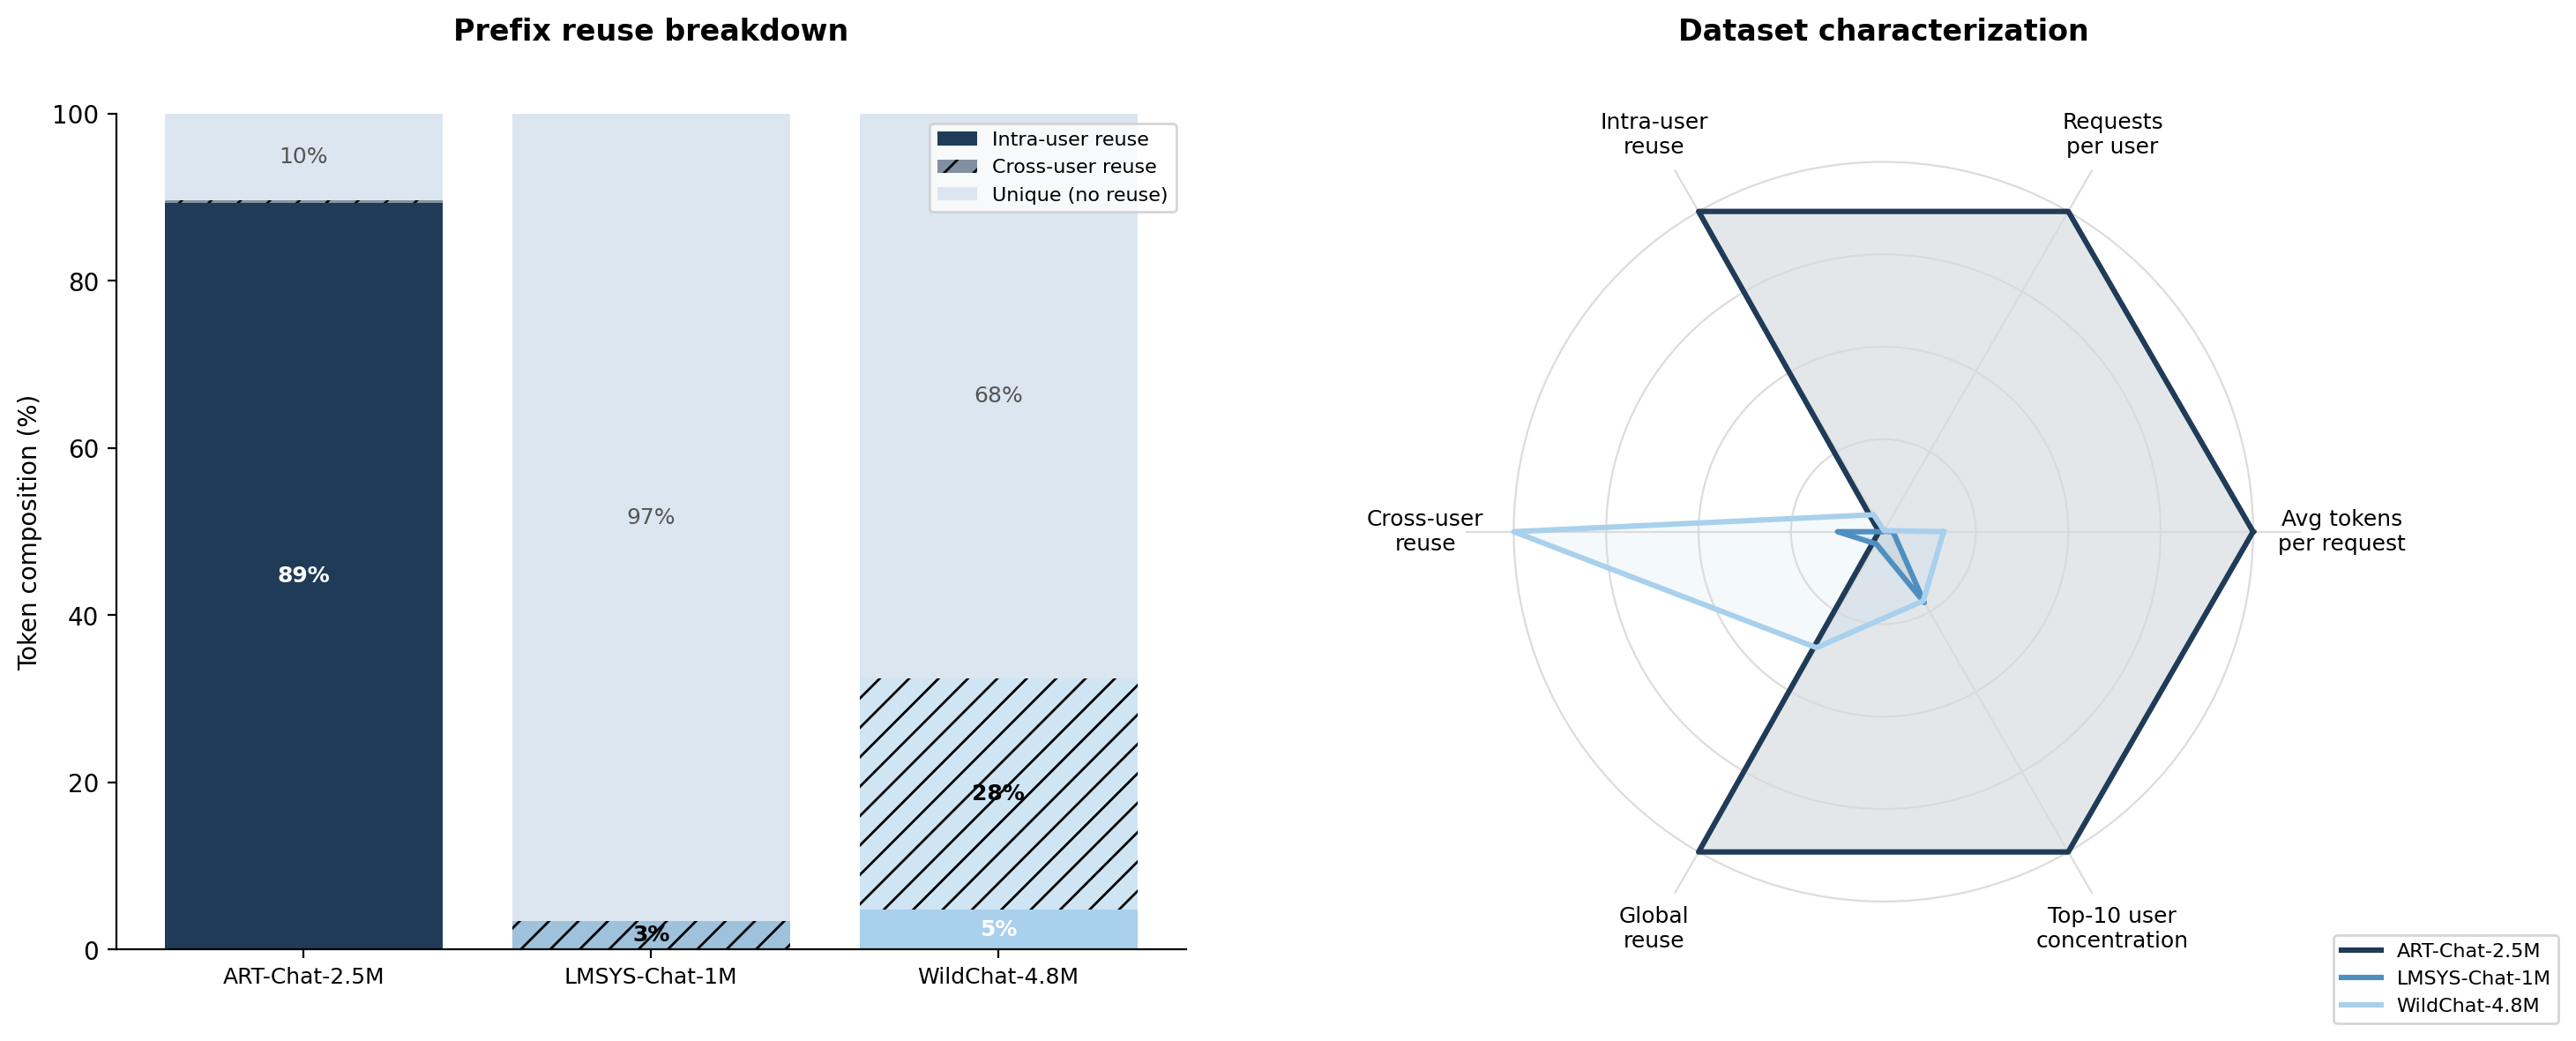
\includegraphics[width=\linewidth]{dataset_combined.png}
\caption{\textit{Left}: Dataset characterization. ART-Chat-2.5M's prefix reuse
  is overwhelmingly intra-user (89\%) with minimal cross-user reuse (0.3\%), which reflects
  the long-context, multi-turn data; WildChat's prefix reuse is predominantly cross-user (28\%, shared templates); LMSYS
  has minimal cross-user reuse (3\%) and no intra-user reuse due to the lack of a field for client origin. \textit{Right}: ART-Chat-2.5M
  contains the maximum for each attribute except for cross-user reuse, which in WildChat is a function of the shorter average token length (2,925 tokens) and a common system prompt.}
\label{fig:dataset_combined}
\end{figure}

\FloatBarrier
\section{Evaluation window characteristics}
\label{app:windows}

\begin{table}[h]
\centering
\small
\caption{Workload characteristics of the tuning and held-out windows.
  Apr~7 is reported in Appendix~\ref{app:apr7}.}
\label{tab:windows}
\begin{tabular}{lrrr}
\toprule
 & Apr5 tuning & Apr6 eval & Apr7 eval \\
 & 16:15--16:45 & 15:05--15:35 & 19:45--20:15 \\
\midrule
Distinct users               & 579      & 606      & 540      \\
Requests / user              & 12.8     & 12.9     & 16.4     \\
Avg turns / conv.  & 30.3     & 27.7     & 21.5     \\
Multi-turn requests & 73.9\%  & 74.1\%   & 73.7\%   \\
Median input tokens          & 5{,}638  & 5{,}787  & 5{,}745  \\
Avg input tokens             & 6{,}877  & 7{,}008  & 7{,}148  \\
p95 input tokens             & 19{,}886 & 20{,}974 & 20{,}435 \\
Block global reuse           & 78.8\%   & 77.6\%   & 87.9\%   \\
Block intra-user reuse       & 78.5\%   & 77.1\%   & 87.4\%   \\
\bottomrule
\end{tabular}
\end{table}

\section{Evolutionary strategy convergence}
\label{app:es}

\begin{figure}[ht]
\centering
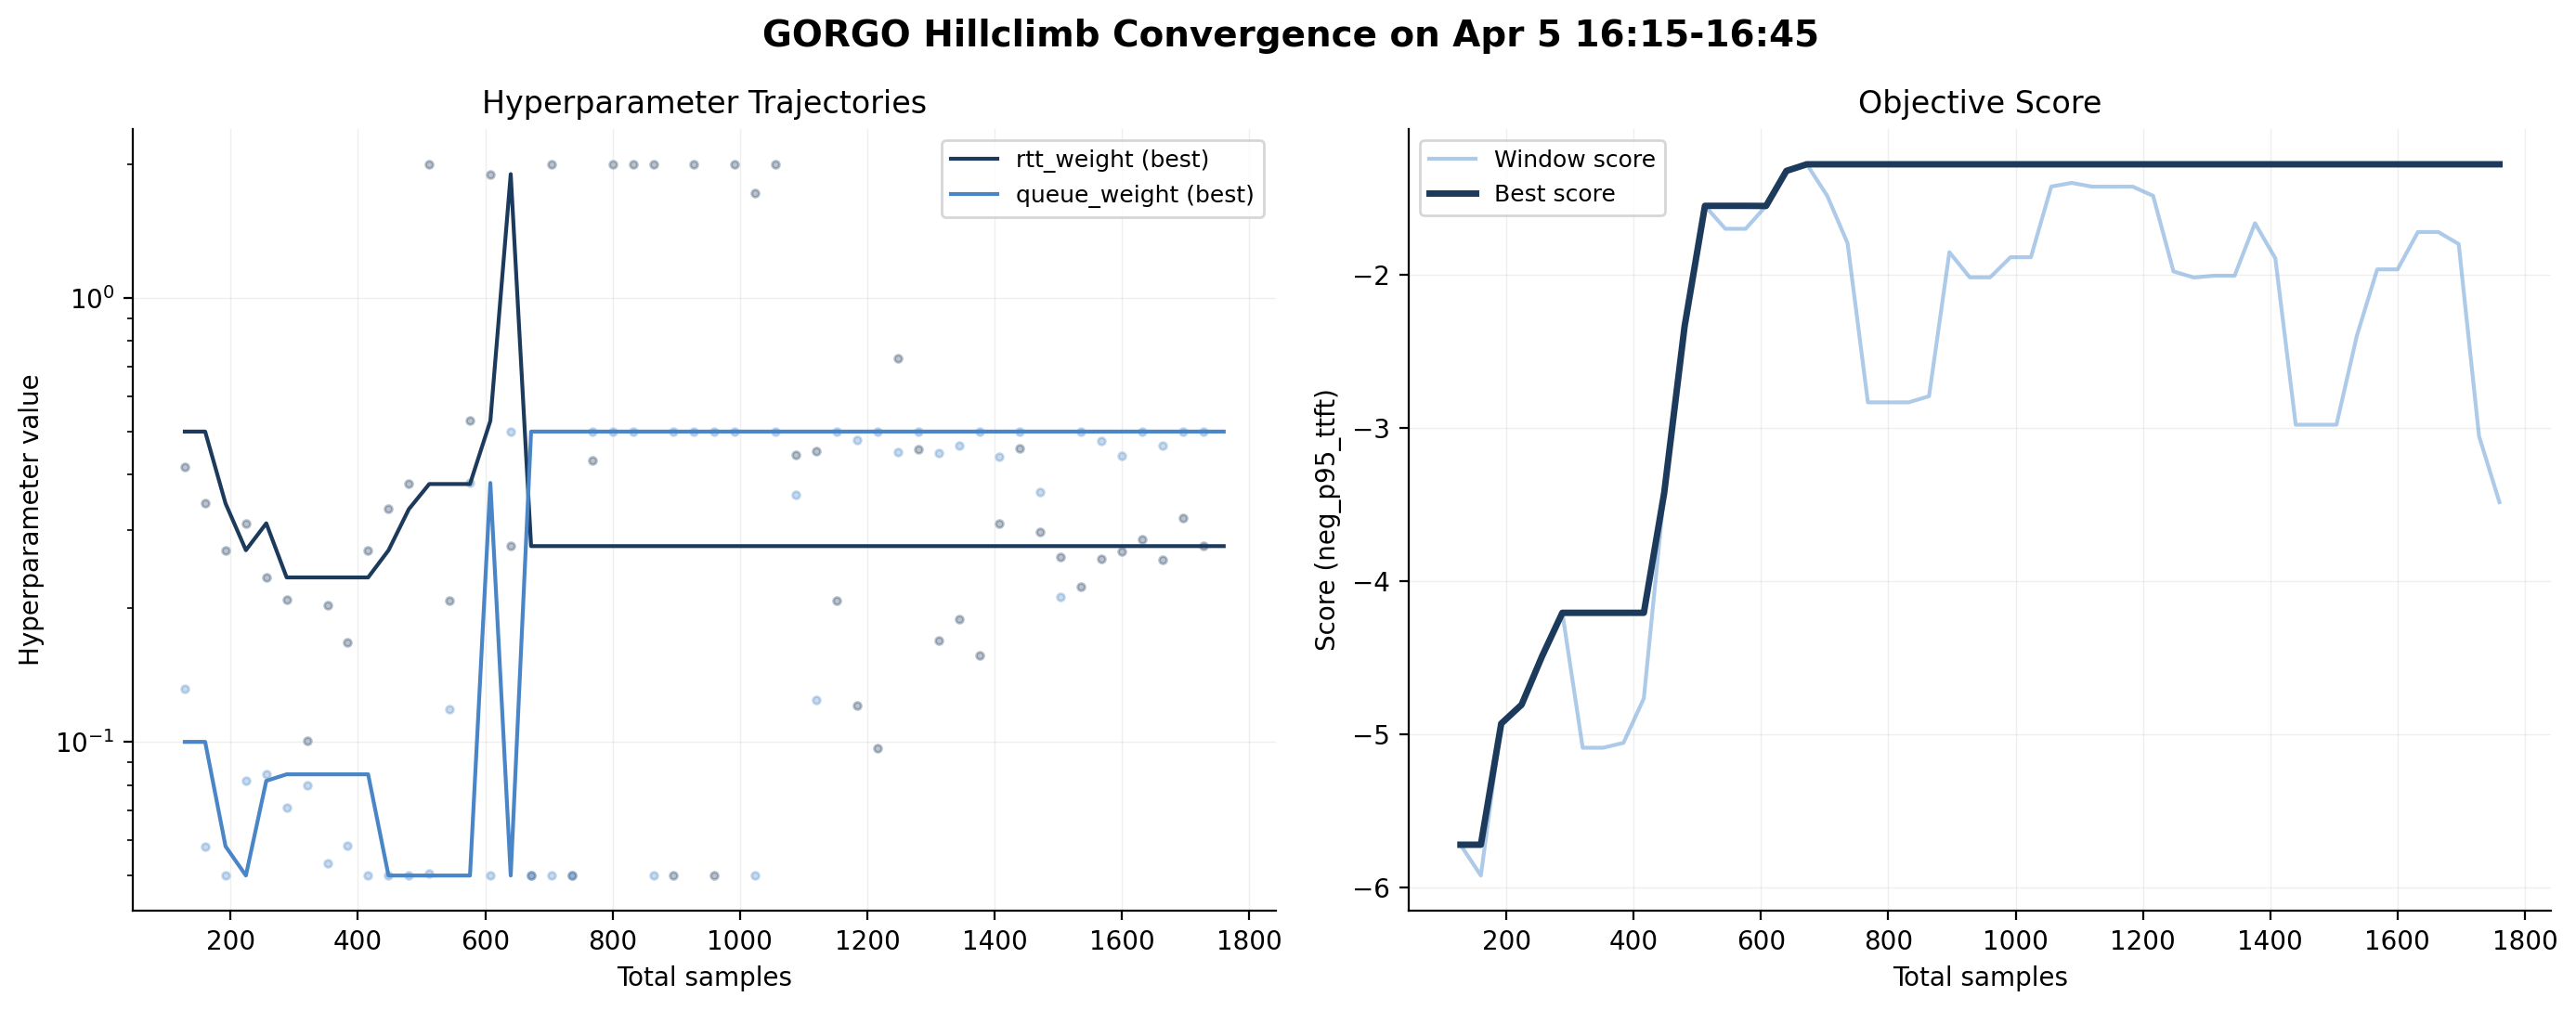
\includegraphics[width=\linewidth]{tune_convergence_2d_v9.png}
\caption{Convergence of the evolutionary strategy on GORGO policy weights $w_{\mathrm{queue}}$ and $w_{\mathrm{rtt}}$.
Both weights reach their local optima after 672 samples, which occurs on the 18th evolutionary step. The fitness function is the negative p95 TTFT (in seconds) of the rolling 128-request tuning window, so a smaller magnitude is better; the best score reached is $-1.276$, i.e.\ a 1.276\,s best-window p95. Because it is computed over the rolling tuning window, this is lower than the 2{,}514\,ms overall tuning-window p95 in Table~\ref{tab:results}.}
\label{fig:es_convergence}
\end{figure}

\FloatBarrier
\section{Apr~7 held-out window}
\label{app:apr7}

\begin{table}[h]
\centering
\small
\setlength{\tabcolsep}{2.7pt}
\caption{Apr~7 19:45--20:15 held-out window.}
\label{tab:apr7_ts3}
\begin{tabular}{lrrrrrrr}
\toprule
Policy & TTFT p50 (ms) & TTFT p95 & TTFT p99 & E2E p50 (s) & E2E p95 & E2E p99 & ITL (ms) \\
\midrule
\textbf{GORGO}          & \textbf{398} & \textbf{1{,}417} & \textbf{2{,}061} & \textbf{1.74}  & \textbf{3.36}  & 6.81           & \textbf{9.3} \\
simple-session-affinity & 457          & 1{,}522          & 2{,}402          & \textbf{1.74}  & 3.92           & 7.12           & \textbf{9.3} \\
least-load              & 495          & 1{,}669          & 2{,}368          & 1.95           & 4.07           & \textbf{6.22}  & 10.0 \\
least-request           & 527          & 1{,}759          & 2{,}578          & 1.98           & 4.44           & 7.85           & 10.0 \\
prefix-cache            & 533          & 1{,}861          & 2{,}872          & 2.20           & 12.00          & 20.04          & 11.8 \\
\bottomrule
\end{tabular}
\end{table}

\section{WildChat replay}
\label{app:wildchat}

\begin{table}[htbp]
\centering
\small
\caption{Held-out WildChat-4.8M replay
(5.7 requests/s open-loop), $c{=}64$, using one H100 replica in each of
us-west4, CANADA-2, and sines-2. Fixed-weight GORGO uses weights learned on
the first window ($w_{\mathrm{rtt}}{=}2.0$,
$w_{\mathrm{queue}}{=}0.104$). Each arm contains 20{,}422 completed requests
with zero failures. Bold marks the best value per column; ITL is the median.}
\label{tab:wildchat}
\setlength{\tabcolsep}{2.7pt}
\begin{tabular}{lrrrrrrr}
\toprule
Policy & TTFT p50 (ms) & TTFT p95 & TTFT p99 & E2E p50 (s) & E2E p95 & E2E p99 & ITL (ms) \\
\midrule
GORGO  & \textbf{215} & \textbf{506} & \textbf{728}   & 1.55          & \textbf{2.42} & \textbf{2.98} & 10.1 \\
random & 244          & 611          & 1{,}166         & \textbf{1.38} & 2.51          & 4.04          & \textbf{8.4} \\
\bottomrule
\end{tabular}
\end{table}

\section{Load weight adaptation}
\label{app:load_ablation}

Table~\ref{tab:load_ablation} and Figure~\ref{fig:load_ablation} give the Apr~2 window where $w_{\mathrm{queue}}{=}0$ routes $\sim$100\% of traffic to one replica. Tuned \texttt{gorgo-static} wins every TTFT percentile but is worst on E2E and ITL tails.

\begin{table}[h]
\centering
\small
\caption{Reward hacking on the Apr~2 12:30--13:00 window. With $w_{\mathrm{queue}}{=}0$, tuned \texttt{gorgo-static} wins every TTFT percentile but is worst on E2E and ITL tails, because it routes $\sim$100\% of traffic to one replica. Bold marks the best value per column; ITL is the median.}
\label{tab:load_ablation}
\setlength{\tabcolsep}{2.7pt}
\begin{tabular}{lrrrrrrr}
\toprule
Policy & TTFT p50 (ms) & TTFT p95 & TTFT p99 & E2E p50 (s) & E2E p95 & E2E p99 & ITL (ms) \\
\midrule
\multicolumn{8}{l}{\textit{Held-out eval --- Apr~2 12:30--13:00 (3{,}071 requests)}} \\
\midrule
gorgo-static (hacked)            & \textbf{180} & \textbf{1{,}072} & \textbf{1{,}810} & 2.05          & 12.49         & 16.63         & 14.1 \\
simple-session-affinity          & 268          & 1{,}715          & 2{,}947          & 1.74          & 3.88          & 5.90          & 10.8 \\
least-load                       & 278          & 1{,}669          & 2{,}665          & 1.69          & 3.89          & 8.94          & 10.1 \\
least-request                    & 274          & 1{,}285          & 1{,}902          & \textbf{1.37} & \textbf{2.61} & \textbf{3.34} & 8.6 \\
random                           & 283          & 1{,}456          & 2{,}124          & 1.40          & 2.92          & 4.24          & \textbf{8.5} \\
prefix-cache                     & 288          & 1{,}468          & 2{,}374          & 1.56          & 3.59          & 7.12          & 9.4 \\
\bottomrule
\end{tabular}
\end{table}

\begin{figure}[ht]
\centering
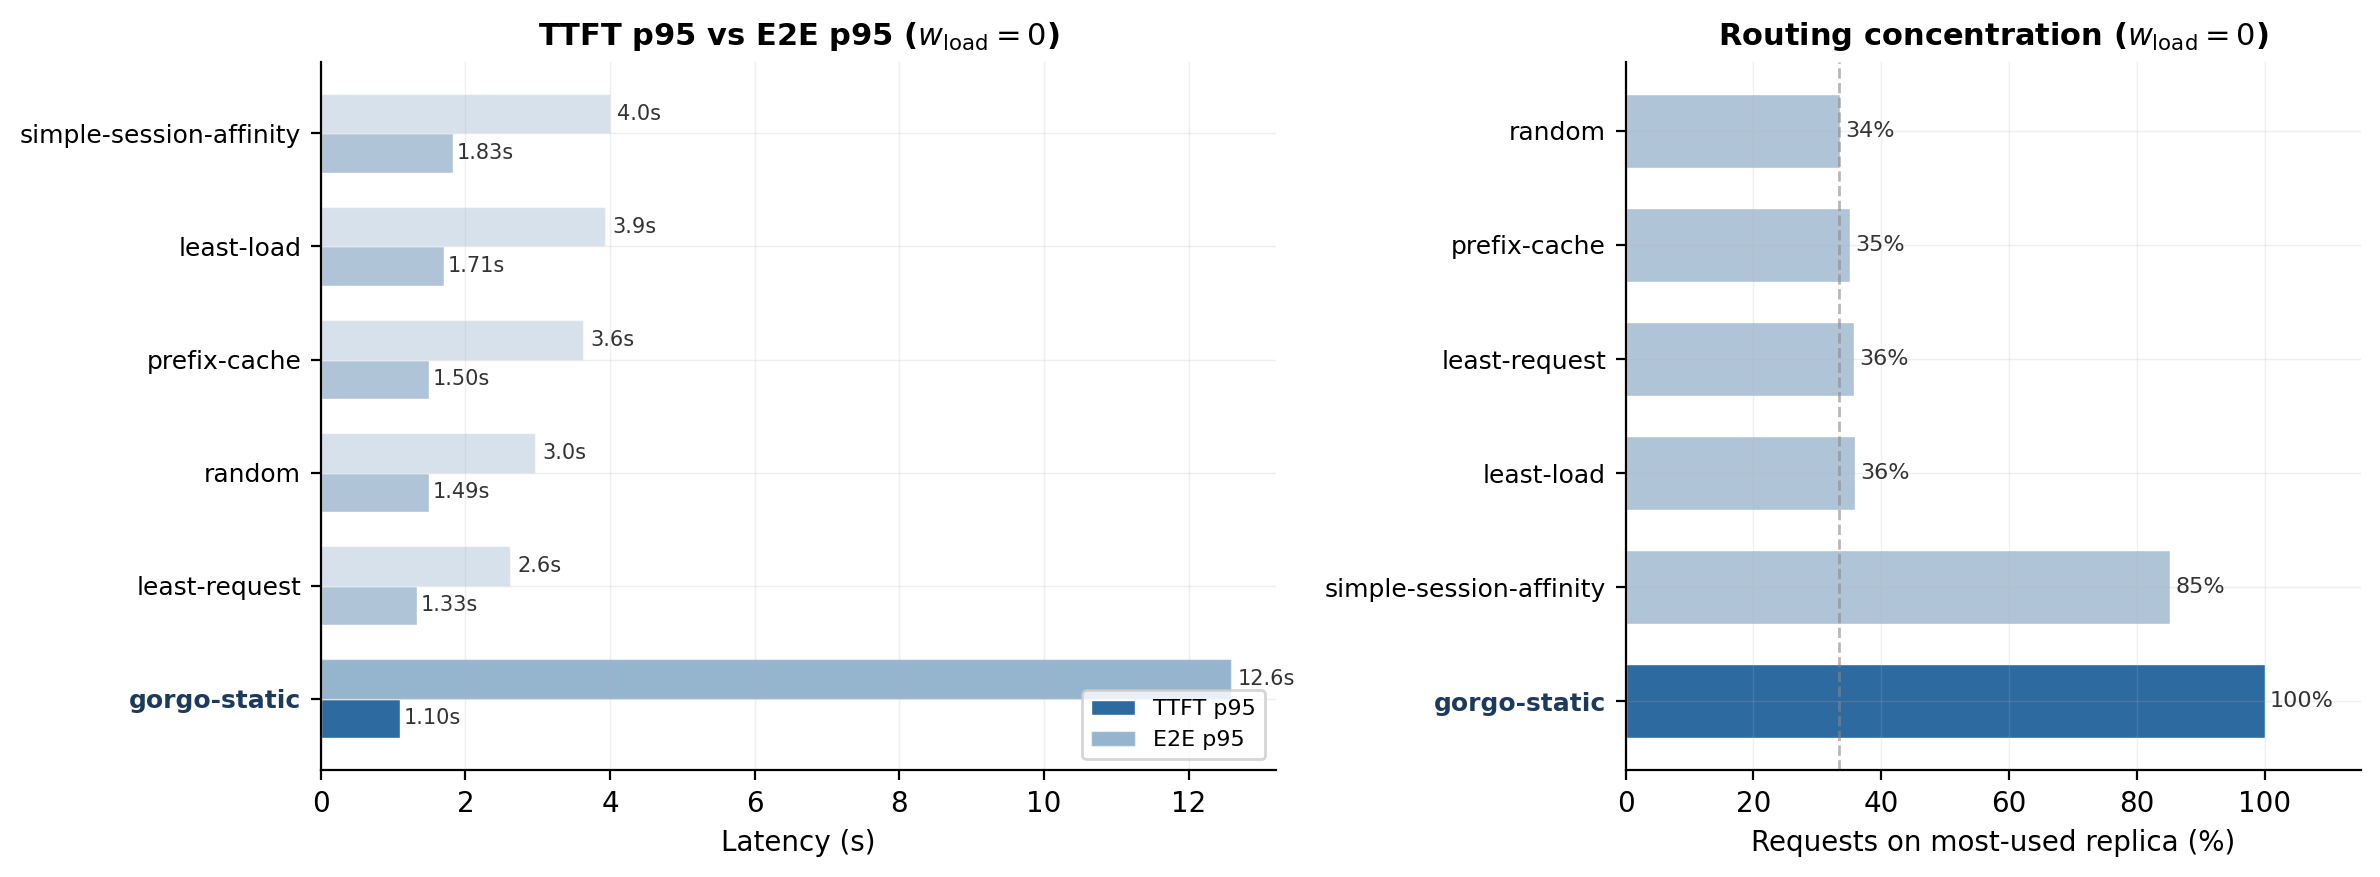
\includegraphics[width=\linewidth]{load_weight_ablation.png}
\caption{\textit{Left}: TTFT p95 (dark) vs.\ E2E p95 (light) on the midday
  diurnal trace with $w_{\mathrm{queue}}{=}0$. \texttt{gorgo-static} wins
  TTFT but its E2E inflates to 12.6\,s. \textit{Right}: routing concentration.
  \texttt{gorgo-static} sends 100\% of requests to one replica.}
\label{fig:load_ablation}
\end{figure}

\end{document}
